\documentclass[10pt,twocolumn]{article}
\usepackage[letterpaper,top=0.68in,bottom=0.72in,left=0.67in,right=0.67in,columnsep=0.24in]{geometry}
\usepackage[T1]{fontenc}
\usepackage{newtxtext,newtxmath}
\usepackage{microtype}
\usepackage{indentfirst}
\usepackage{graphicx}
\usepackage{booktabs}
\usepackage{amsmath}
\usepackage{cite}
\usepackage{enumitem}
\usepackage{caption}
\usepackage{fancyhdr}
\usepackage{lastpage}
\usepackage{balance}
\usepackage{eso-pic}
\usepackage{float}
\usepackage[hidelinks]{hyperref}
\usepackage{xcolor}

\definecolor{paperblack}{RGB}{0,0,0}
\color{paperblack}
\hypersetup{
  pdftitle={Temporal Analysis of API Call Patterns for Early Detection of Malicious Behaviour},
  pdfauthor={Stuart Asiimwe},
  pdfsubject={Author Manuscript},
  pdfkeywords={Malware Detection, API Call Sequence Analysis, Temporal Analysis, Dynamic Malware Analysis, Behavioural Analysis, Early Detection},
  colorlinks=false
}
\captionsetup{font=small,labelfont=bf,labelsep=period}
\setlength{\parindent}{1em}
\setlength{\parskip}{0pt}
\setlength{\columnsep}{0.24in}
\hyphenpenalty=10000
\exhyphenpenalty=10000
\emergencystretch=1.5em
\raggedbottom
\pagestyle{fancy}
\fancyhf{}
\renewcommand{\headrulewidth}{0pt}
\renewcommand{\footrulewidth}{0pt}
\fancyfoot[C]{\footnotesize \thepage}
\setlength{\footskip}{22pt}

\title{\vspace{-1.8em}\bfseries\LARGE Temporal Analysis of API Call Patterns for Early Detection of Malicious Behaviour}
\author{\normalsize\textbf{Stuart Asiimwe}\\[-1pt]
\small Department of Computer Science and Software,\\
\small Hanyang University, Seoul, South Korea\\
\small \href{mailto:stuart@hanyang.ac.kr}{stuart@hanyang.ac.kr}}
\date{\small Author Manuscript - October 2024}

\begin{document}
\AddToShipoutPictureBG{%
  \AtPageCenter{%
    \makebox[0pt][c]{%
      
\includegraphics[width=245pt]{assets/hanyang-university-symbol-watermark.png}%
    }%
  }%
}
\maketitle
\thispagestyle{fancy}

\begin{abstract}
\hspace*{\parindent}This paper evaluates early malware detection from partial Windows API-call sequences. After exact duplicates and conflicting labels are removed, 13,191 unique traces are divided into fixed training, validation, and test sets. A call-frequency baseline is compared with an order-aware unigram-bigram model using class-weighted logistic regression.

\hspace*{\parindent}The order-aware model achieves 0.818 balanced accuracy and 0.919 ROC-AUC after 20 calls, reaching 0.904 balanced accuracy after 80 calls. The validation-selected sequential policy detects 83.6\% of malicious traces by 100 calls with a 5.4\% benign false-alarm rate.

\hspace*{\parindent}On the held-out test set, partial API-call sequences distinguish malicious from benign traces. Deduplication reduces the risk that repeated sequences inflate the reported performance estimates.
\end{abstract}

\noindent\textbf{Keywords:} malware detection; API-call sequences; temporal analysis; dynamic analysis; behavioural analysis; early detection

\section{Introduction}
Dynamic malware analysis records how a program interacts with an operating system during execution. Windows API calls capture activities such as process creation, file access, registry modification, memory allocation, and network communication. Because these calls accumulate over time, a practical detector should identify malicious activity before the full trace is available. Previous studies have used API-call sequences to classify Windows malware \cite{catak2019,tang2019} and to make decisions from partial sequences \cite{maniriho2024}.

Here, ``early'' refers to the number of calls observed rather than elapsed time. The analysis addresses 3 questions:
\begin{enumerate}[label=(\arabic*),leftmargin=2.2em,itemsep=1pt,topsep=2pt]
 \item How does detection quality change as the observed prefix grows from 5 to 100 calls?
 \item Does local call order improve on call-frequency features?
 \item How early can a sequential policy alert while controlling benign false alarms?
\end{enumerate}

The main contribution is an evaluation designed to prevent sequence leakage. Exact duplicates and label conflicts are resolved before partitioning, models and thresholds are selected on validation data, and the test partition is reserved for final evaluation. This design addresses known sources of experimental bias in malware research \cite{pendlebury2019}.

\section{Dataset Audit}
The analysis uses the public \emph{Malware Analysis Datasets: API Call Sequences} collection \cite{oliveira2019}. Each row contains a file hash, a binary label, and the first 100 consecutive non-repeated calls made by the parent process in a Cuckoo Sandbox report. The raw table contains 43,876 rows: 42,797 malware traces and 1,079 benign traces.

For a sequence $x_i=(a_{i,1},\ldots,a_{i,100})$, an exact fingerprint is computed as
\begin{equation}
 h_i=\operatorname{SHA256}(a_{i,1}\Vert\cdots\Vert a_{i,100}),
 \label{eq:hash}
\end{equation}
where $\Vert$ denotes deterministic concatenation. The audit identifies 13,206 distinct fingerprints and 30,670 rows that duplicate another complete sequence. 15 fingerprint groups, covering 1,641 rows, contain both labels. These groups are removed because the available data cannot establish the correct label, and 1 row is retained from each remaining group. This process yields 13,191 unique traces: 12,582 malware and 609 benign.

The cleaned data remain strongly imbalanced. Class weights are computed from the training partition as
\begin{equation}
 \omega_c=\frac{N}{2N_c},
 \label{eq:weights}
\end{equation}
where $N$ is the number of training observations and $N_c$ is the number in class $c$. This avoids synthesising or repeatedly sampling minority observations.

\section{Method}
\subsection{Data Partitions}
The deduplicated data are divided into stratified training, validation, and test partitions of 70\%, 15\%, and 15\%, respectively, using seed 20241022. Deduplication occurs first, so a complete sequence cannot appear in more than 1 partition. The validation partition is used to select regularisation and thresholds, and the test partition is evaluated once after these choices are fixed.

For the call budgets $\mathcal{K}=\{5,10,20,40,60,80,100\}$, each trace produces the prefix
\begin{equation}
 x_i^{(k)}=(a_{i,1},\ldots,a_{i,k}),\qquad k\in\mathcal{K}.
 \label{eq:prefix}
\end{equation}
A separate model is fitted at each checkpoint. A result at $k$ therefore measures classification performance using exactly the first $k$ calls.

\subsection{Feature Representation}
The frequency baseline represents API identifier $j$ by its normalised count:
\begin{equation}
 f_{i,j}^{(k)}=\frac{1}{k}\sum_{t=1}^{k}\mathbb{I}(a_{i,t}=j).
 \label{eq:frequency}
\end{equation}
This records which calls occurred while discarding their order. The order-aware model uses the feature multiset
\begin{equation}
 \phi(x_i^{(k)})=\{a_{i,t}\}_{t=1}^{k}\cup
 \{(a_{i,t},a_{i,t+1})\}_{t=1}^{k-1},
 \label{eq:ngrams}
\end{equation}
This multiset is mapped to a deterministic 32,768-dimensional sparse vector by feature hashing and then normalised to unit $L_2$ length. Let $\mathbf{z}_i^{(k)}$ denote the frequency vector in Eq.~\eqref{eq:frequency} for the baseline or the hashed vector derived from Eq.~\eqref{eq:ngrams} for the order-aware model.

Each representation is supplied to a class-weighted, $L_2$-regularised logistic regression classifier \cite{pedregosa2011}. At checkpoint $k$, the predicted probability of malware is
\begin{equation}
 \hat p_i^{(k)}=\sigma\!\left(\mathbf{w}_k^\top\mathbf{z}_i^{(k)}+b_k\right),
 \quad \sigma(z)=\frac{1}{1+e^{-z}}.
 \label{eq:logistic}
\end{equation}
The tested inverse regularisation strengths are $C\in\{0.1,1,10\}$. The value with the highest validation macro F1 is selected, with validation balanced accuracy used to break ties.

\subsection{Alert Thresholds}
For each checkpoint and candidate false-positive limit $\alpha\in\mathcal{A}=\{0,0.01,0.02,0.05\}$, the validation threshold maximises malware true-positive rate subject to that limit:
\begin{equation}
 \tau_{k,\alpha}^*=\arg\max_{\tau}\operatorname{TPR}_{\rm val}(\tau)
 \quad\text{s.t.}\quad \operatorname{FPR}_{\rm val}(\tau)\leq\alpha.
 \label{eq:threshold}
\end{equation}
Continuous-monitoring candidates require $r\in\{1,2,3\}$ consecutive positive checkpoints. An alert at checkpoint $k_j$ occurs when
\begin{equation}
 A_i(k_j;r,\alpha)=\prod_{q=0}^{r-1}
 \mathbb{I}\!\left(\hat p_i^{(k_{j-q})}\geq\tau_{k_{j-q},\alpha}^*\right)=1.
 \label{eq:alert}
\end{equation}
The pair $(r^*,\alpha^*)$ is selected to maximise malware coverage while keeping the cumulative validation false-alarm rate at or below 5\%. The selected values, $(3,0.05)$, are applied unchanged to the test set.

\subsection{Metrics}
Because 95.4\% of cleaned observations are malware, accuracy alone is misleading. Balanced accuracy is
\begin{equation}
 \operatorname{BAcc}=\tfrac{1}{2}(\operatorname{TPR}+\operatorname{TNR}),
 \label{eq:bacc}
\end{equation}
Macro F1 is the unweighted mean of the malware and benign F1 scores. Reported measures also include ROC-AUC, malware recall, benign specificity, false-positive rate, and precision-recall area for each class. 95\% confidence intervals for balanced accuracy, macro F1, and ROC-AUC are estimated from 1,000 stratified bootstrap samples of the fixed test set.

\section{Results}
\subsection{Prefix Classification}
The order-aware representation outperforms the frequency baseline at every checkpoint (Table~\ref{tab:prefix}). At 20 calls it reaches 0.818 balanced accuracy (95\% CI 0.785-0.847) and 0.919 ROC-AUC (95\% CI 0.894-0.939). Malware recall is 0.734 and benign specificity is 0.902 at the validation-selected operating threshold.

At 40 calls, balanced accuracy rises to 0.870 (95\% CI 0.839-0.896), ROC-AUC to 0.946 (95\% CI 0.926-0.962), malware recall to 0.816, and specificity to 0.924. The 80-call model achieves the highest balanced accuracy, at 0.904 (95\% CI 0.878-0.927). Its ROC-AUC is 0.965, malware recall is 0.862, and specificity is 0.946.

\begin{table*}[t]
\centering
\caption{Test performance by observed API-call budget. Thresholded measures use validation-selected thresholds.}
\label{tab:prefix}
\small
\begin{tabular}{rrrrrr}
\toprule
Calls & Frequency BAcc & Order BAcc & Order ROC-AUC & Malware recall & Benign specificity\\
\midrule
5   & 0.539 & 0.586 & 0.857 & 0.216 & 0.957\\
10  & 0.560 & 0.614 & 0.866 & 0.282 & 0.946\\
20  & 0.760 & 0.818 & 0.919 & 0.734 & 0.902\\
40  & 0.695 & 0.870 & 0.946 & 0.816 & 0.924\\
60  & 0.793 & 0.853 & 0.948 & 0.858 & 0.848\\
80  & 0.838 & \textbf{0.904} & \textbf{0.965} & 0.862 & 0.946\\
100 & 0.865 & 0.897 & 0.964 & 0.826 & 0.967\\
\bottomrule
\end{tabular}
\end{table*}

\begin{figure*}[t]
 \centering
 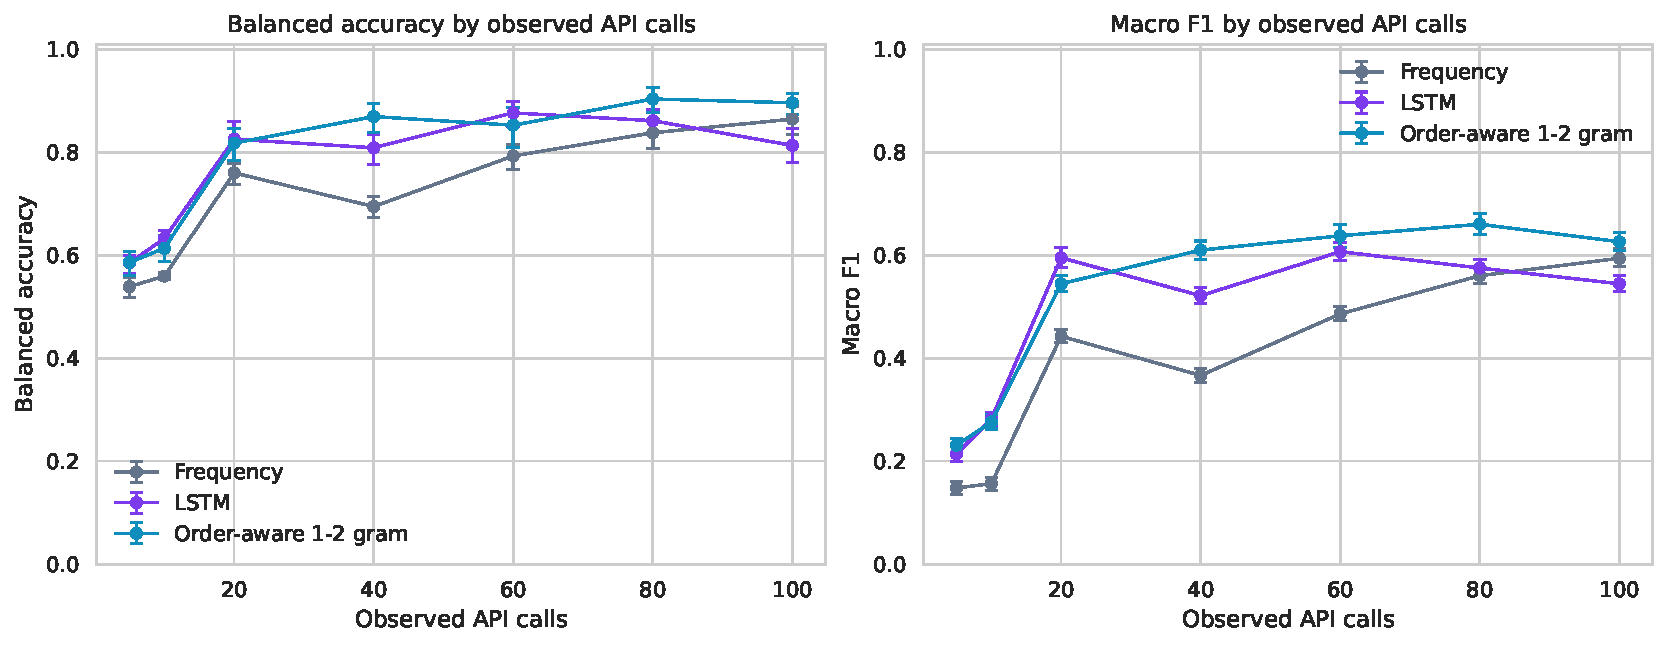
\includegraphics[width=0.82\textwidth]{../results/figures/prefix_performance.pdf}
 \caption{Prefix performance. Shaded bands and error bars show 95\% stratified bootstrap intervals on the fixed test partition.}
 \label{fig:prefix}
\end{figure*}

Performance is not monotonic across checkpoints. Each prefix model is fitted independently, and each operating threshold is selected on a small benign validation subset. The 80-call model produced the highest test balanced accuracy, but this does not establish a monotonic relationship between prefix length and performance.

\begin{figure*}[t]
 \centering
 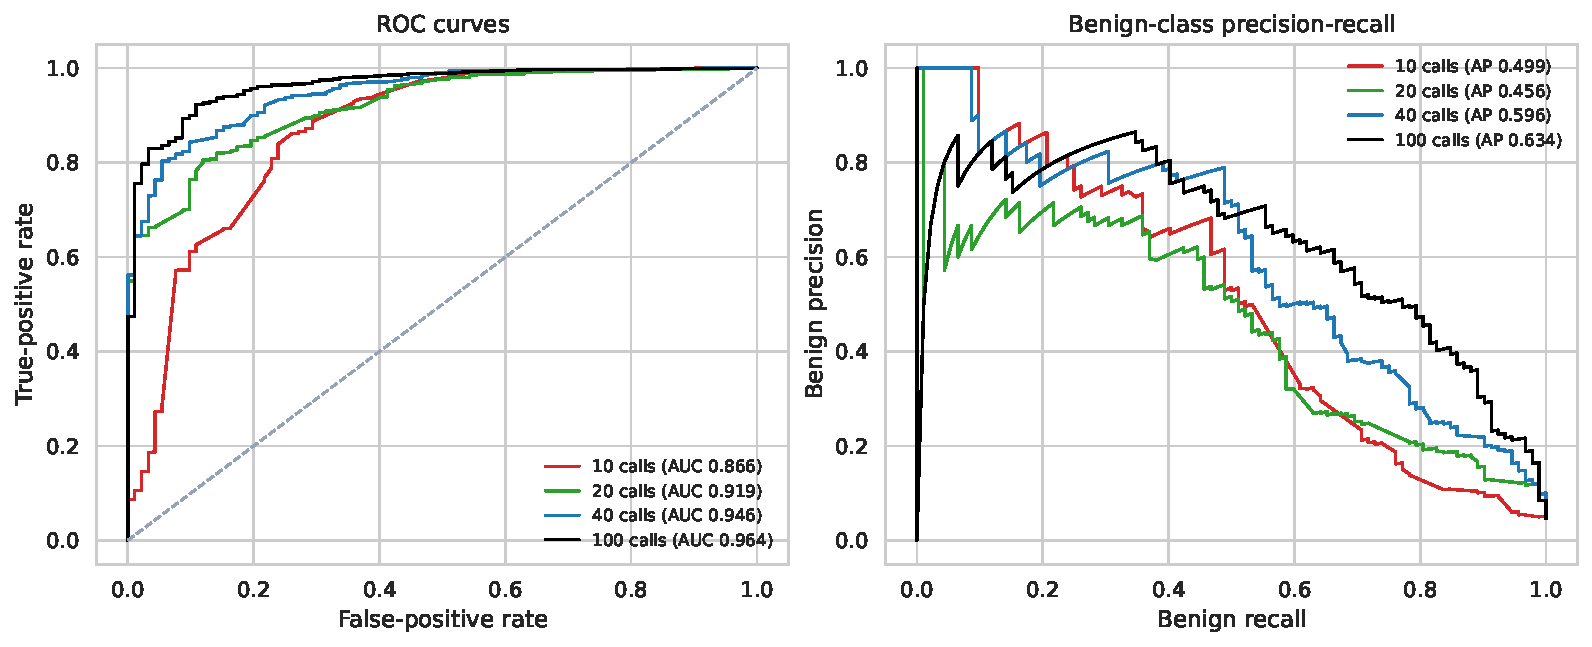
\includegraphics[width=0.86\textwidth]{../results/figures/roc_pr_curves.pdf}
 \caption{ROC and benign-class precision-recall curves for the order-aware model at selected checkpoints.}
 \label{fig:curves}
\end{figure*}

\subsection{Early-Detection Policy}
The validation-selected policy requires 3 consecutive positive checkpoints. On the test set, it detects 16.3\% of malware by 20 calls, 71.9\% by 60 calls, 80.2\% by 80 calls, and 83.6\% by 100 calls. Among detected malware, the median alert occurs at 60 calls. 5 of 92 benign test traces trigger an alert, giving a cumulative false-alarm rate of 5.4\%.

For a call budget $k$, malware detection coverage is
\begin{equation}
 D(k)=\frac{\sum_{i:y_i=1}\mathbb{I}(T_i\leq k)}{\sum_i\mathbb{I}(y_i=1)},
 \label{eq:coverage}
\end{equation}
where $T_i$ is the first checkpoint satisfying Eq.~\eqref{eq:alert}. The cumulative benign false-alarm rate is calculated analogously over traces for which $y_i=0$.

\begin{table}[t]
\centering
\caption{Cumulative sequential-policy outcomes.}
\label{tab:policy}
\small
\begin{tabular}{rrr}
\toprule
Calls & Malware detected & Benign false alarms\\
\midrule
20  & 16.3\% & 2.2\%\\
40  & 25.4\% & 4.3\%\\
60  & 71.9\% & 4.3\%\\
80  & 80.2\% & 4.3\%\\
100 & 83.6\% & 5.4\%\\
\bottomrule
\end{tabular}
\end{table}

\subsection{Evaluation Constraints}
\subsubsection{Sequence Integrity}
A conventional stratified 80/20 row split of the original data causes 73.7\% of test rows to duplicate a sequence in the training set. With this split, the order-aware model reports 0.976 ROC-AUC and 93.4\% accuracy. These values exceed the strict deduplicated estimates, but most test rows no longer represent unseen behaviour. This comparison shows why sequence-level deduplication must occur before evaluation.

Exact duplicate removal prevents direct sequence leakage, but near-duplicate variants may remain. Family labels are unavailable, so related malware samples may still occur in different partitions.

\subsubsection{Model Constraints}
Feature hashing can produce collisions. The unigram-bigram representation captures only local call order, and the linear classifier cannot model longer dependencies directly. Threshold selection also relies on a limited benign validation sample.

\subsubsection{Generalisability}
The results are derived from 1 public sandbox dataset and may not transfer directly to other operating systems, sandbox configurations, or deployment environments. Because the dataset lacks collection dates and malware-family labels, chronological and family-held-out evaluation is not possible.

\subsubsection{Measurement Boundaries}
The source data contain no timestamps, so elapsed detection time cannot be estimated. Call count measures how much of a trace the model has observed. The reported false-alarm rate applies to individual traces in this dataset, rather than to hosts or days in a deployed system.

\section{Discussion}
The models distinguish malicious from benign traces before all 100 calls are observed. The representation that includes local call order performs better than normalised call frequencies at every tested budget.

The sequential policy delays an alert until 3 consecutive checkpoints are positive; among detected malware, the median alert occurs at 60 calls. These results establish performance on progressively longer prefixes within this dataset.

\begin{figure}[H]
 \centering
 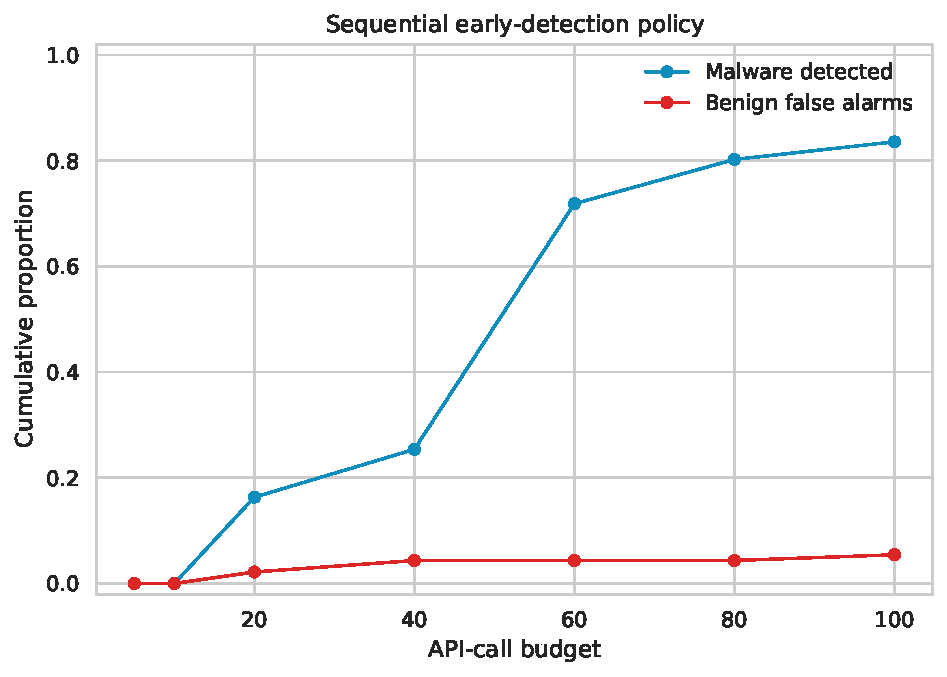
\includegraphics[width=\columnwidth]{../results/figures/early_detection_policy.pdf}
 \caption{Cumulative malware detection and benign false alarms by call budget.}
 \label{fig:policy}
\end{figure}

\section{Conclusion}
The results show that malicious Windows behaviour can be detected before a complete API-call trace is available. The order-aware unigram-bigram model achieves 0.818 balanced accuracy at 20 calls and 0.904 at 80 calls. The sequential policy detects 71.9\% of malicious traces by 60 calls and 83.6\% by 100 calls, with a 5.4\% benign false-alarm rate.

In future work, I plan to evaluate chronologically collected traces, hold out complete malware families, and include more benign samples. I also want to work with data that retain repeated calls and timestamps, then compare lightweight sequential methods with recurrent and transformer models using the same deduplication, validation, and held-out test procedure.

\subsection*{Artifacts}
The experiment code, configuration, and results are available in the project repository \cite{asiimwe2024repository}.

\clearpage
\begin{thebibliography}{9}
\bibitem{oliveira2019} A. Oliveira, ``Malware Analysis Datasets: API Call Sequences,'' \emph{IEEE DataPort}, 2019.
\bibitem{catak2019} F. O. Catak and A. F. Yazı, ``A benchmark API call dataset for Windows PE malware classification,'' \emph{arXiv preprint arXiv:1905.01999}, 2019.
\bibitem{pendlebury2019} F. Pendlebury, F. Pierazzi, R. Jordaney, J. Kinder, and L. Cavallaro, ``TESSERACT: Eliminating experimental bias in malware classification across space and time,'' in \emph{Proc. 28th USENIX Security Symp.}, 2019, pp. 729-746.
\bibitem{maniriho2024} P. Maniriho, A. N. Mahmood, and M. J. M. Chowdhury, ``EarlyMalDetect: A novel approach for early Windows malware detection based on sequences of API calls,'' \emph{arXiv preprint arXiv:2407.13355}, 2024.
\bibitem{tang2019} M. Tang and Q. Qian, ``Dynamic API call sequence visualisation for malware classification,'' \emph{IET Information Security}, vol. 13, no. 4, pp. 367-377, 2019.
\bibitem{pedregosa2011} F. Pedregosa \emph{et al.}, ``Scikit-learn: Machine learning in Python,'' \emph{Journal of Machine Learning Research}, vol. 12, pp. 2825-2830, 2011.
\bibitem{asiimwe2024repository} S. Asiimwe, ``API Call Patterns,'' GitHub repository, 2024. \url{https://github.com/stuartasiimwe7/api-call-patterns}
\end{thebibliography}

\end{document}
